\documentclass[11pt]{article}

\usepackage[T1]{fontenc}
\usepackage[utf8]{inputenc}
\usepackage{fullpage}
\usepackage{graphicx}
\usepackage[hidelinks]{hyperref}
\usepackage{parskip}
\renewcommand{\familydefault}{pbk}

\begin{document}

\begin{center}
\begin{minipage}[c]{0.42\textwidth}
\centering
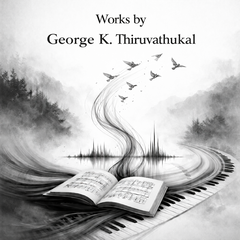
\includegraphics[width=1.45in,height=1.45in,keepaspectratio]{art-song-program-notes-assets/compositions-logo.png}
\end{minipage}
\hspace{0.04\textwidth}
\begin{minipage}[c]{0.42\textwidth}
\centering

\includegraphics[width=1.45in,height=1.45in,keepaspectratio]{art-song-program-notes-assets/site-qr.png}
\end{minipage}

\vspace{1em}

{\LARGE \textbf{Program Notes}}\\[0.5em]
{\Large \textit{We Choose the Moon, We Choose Earth}}\\[0.5em]
{\normalsize George K.\ Thiruvathukal}
\end{center}

\textit{We Choose the Moon, We Choose Earth} is an art song for voice, violin, viola, trumpet, and piano. The piece places John F.\ Kennedy's 1962 Rice University moon speech in conversation with the Artemis II mission, treating space exploration not simply as a historical achievement but as a continuing public ideal. The work asks what it means to choose difficult, collective work in the present tense, and it answers that question by turning the image of the moonshot back toward Earth.

Kennedy's language gives the song its public voice. His words about challenge, resolve, and shared effort shape the opening and the central refrain. The emotional turn comes from Christina Koch's Artemis II statement, ``We choose Earth,'' which shifts the meaning of exploration. In this piece, the moon is not a symbol of escape. It becomes a way of thinking again about responsibility: to one another, to the planet, and to the difficult work of building a more humane future together.

Musically, the score moves between speech-like delivery and more sustained melodic writing. The opening establishes a distant, spacious atmosphere, after which the vocal line enters in a direct, speech-based style. As the refrain unfolds, the harmony opens into brighter jazz-influenced colors and the ensemble becomes more active. A later bridge cools the texture and shifts the perspective toward Artemis II before the ending returns quietly to the shared idea that frames the work: we choose Earth, and we choose each other.

Although the piece began as a broader production concept, the current version is a notated lead-score hybrid written in Abjad and LilyPond. That format preserves clarity of text and form while leaving interpretive space inside the accompaniment and ensemble writing. The result is a score that balances concert-music notation with the directness of song, allowing the political and emotional meaning of the text to emerge through pacing, repetition, and ensemble color rather than through spectacle alone.

\textbf{Duration:} approximately 4 minutes, 13 seconds.

\textbf{Website:} \url{https://compositions.gkt.sh}

\end{document}
